\documentclass[10pt]{article}
\usepackage[a4paper,margin=2cm]{geometry}
\usepackage[T1]{fontenc}
\usepackage{lmodern}
\usepackage{graphicx}
\usepackage{booktabs}
\usepackage{amsmath}
\usepackage[hidelinks]{hyperref}
\usepackage{caption}
\captionsetup{font=small,labelfont=bf}
\setlength{\parskip}{3pt}

\title{Autoresearch on EEG emotion decoding:\\
seventy agent-run experiments scored on new people and new videos}
\author{Mathias Chebbah\\\small HABS Neuro-AI Hackathon, Universit\'e Paris-Saclay, November 2026}
\date{}

\begin{document}
\maketitle

\begin{abstract}
We applied the autoresearch loop of Karpathy (2026) to the HABS multimodal
dataset. An agent edited one model file, scored each version on a fixed
objective, and kept a change only when it beat the current best by at least
0.005. The objective is the within-person Spearman correlation between
predicted and reported valence and arousal, measured only for people and
video themes absent from training. Over 72 experiments on 13,388
development trials, the score rose from 0.030 to 0.105 through four kept changes. They were
training on person-centred ratings, averaging EEG power over six regions,
adding relative band power, and averaging a regional and a channel-level
ridge regression. On a sealed test scored once (55 new people,
21 new themes, 1,174 trials) the final model reached 0.139 (95\% interval
0.083 to 0.196), against 0.083 for the starting model. The paired gain was
+0.056 (+0.012 to +0.101). The development score did not overstate the test
score. Two ablations locate the signal. EEG carried valence and peripheral
signals carried most of the arousal information in development. A model
fitted only on video-averaged physiology scored 0.010, so the information that
transfers to new videos comes from each viewer's trial-level response, not
from a stimulus signature shared across viewers. The effect is small. Pooled
AUCs stay between 0.52 and 0.56.
\end{abstract}

\section{Question}

The HABS release pairs 64-channel EEG, ECG, skin conductance and respiration
with ratings of 10-second emotional videos. Another hackathon team reported
AUCs of 0.58 for arousal and 0.593 for valence on a high/low split (Slack,
10 November). The dataset guide warns that videos recur across people. With a
split by person only, a model can score by recognising a video it has seen in
training. Our earlier study on the same data found that physiology added nothing measurable
to stimulus context and personal calibration when predicting an aversive
rating score. We asked whether physiology predicts a viewer's
rating of a video when both the viewer and the video theme are new to the
model, and how far an automated search can raise that number before it overfits
its own validation set.

\section{Method}

\paragraph{Data.} We used every audited trial: 22,974 trials from 314
participant IDs, 84 themes and 5 cohorts. A single job on the HABS GPU
backend computed 1,180 label-free feature columns per trial (\texttt{extract.py}):
log band power in five bands (1 to 45 Hz) for each EEG channel during the
video and the 2 s before it, five 200-ms evoked bins, a 20-channel covariance,
heart rate and its change, skin-conductance level, slope and variability,
and respiratory amplitude and rate. EEG came from the released ICA-cleaned
files for 22,898 trials. We excluded eye tracking, which the organisers
reported as misaligned.

\paragraph{Splits.} A SHA-256 hash places each participant and each theme in
one of five buckets. Bucket 0 of both forms the sealed test (new person, new
theme). Two further test sets share one bucket: test people with other themes
(new person, seen theme) and other people with test themes (seen person, new
theme). The remaining 13,388 trials (259 people, 63 themes) form the
development set. A $3\times3$ blocked cross-fit scores it. Each block of
people fold $p$ and theme fold $t$ is predicted by a model trained on the
other people folds and the other theme folds. Every development prediction
therefore concerns an unseen person watching an unseen theme. The model never
sees the video name, theme, intended emotion or start marker of a row it
predicts, because the marker code also encodes the intended emotion.

\paragraph{Objective.} For each person with at least five varied trials, we
compute Spearman's $\rho$ between predicted and reported rating. The score is
the mean over people, averaged over valence and arousal. Chance is 0. A
person's offset or scale use cannot raise it. We also report pooled AUC for
ratings above 5, for comparison with other teams.

\paragraph{Loop.} Following Karpathy's design, \texttt{prepare.py} (data,
splits, metric, a 420-s fitting budget) is fixed, and \texttt{train.py} is the
only file the agent edits. A GitHub Actions workflow takes \texttt{train.py}
from the experiment commit and every other file from \texttt{main}, so an
experiment cannot change how it is scored. Runs print aggregates only and
trial rows never leave the ephemeral runner. The agent (Claude, directed by
\texttt{program.md}) wrote batches of 2 to 11 variants of the current best,
scored them in parallel, and kept a variant when its gain was at least 0.005,
about half the bootstrap standard error of the score. Ablations and
references were logged but never kept. All 72 experiment commits stay on the
branch \texttt{autoresearch/nov19}. We froze the protocol in the journal
before reading any score. The sealed test ran once, after the search ended,
for the starting model, the final model, two ablations of the final model and
a session-position reference, with 5,000 bootstrap resamples of test people.

\section{Results}

\paragraph{Search.} Figure~\ref{fig:progress} shows the development score of
every experiment. Training on ratings centred on each person's mean gave the
largest step, from 0.030 to 0.085, which matches the within-person objective.
Averaging channels over six regions raised it to 0.090 with fewer features,
relative band power to 0.097, and averaging a regional and a channel-level
ridge to 0.105. A rewrite with identical output became the final model. Many
ideas lowered the score: z-scoring features within person, gradient boosting
(0.051 to 0.076), kernel and quadratic expansions (0.037 to 0.056), the
evoked bins, the covariance tangent space, pre-onset baselines and
hemispheric asymmetry. Wider feature sets lost to narrower ones. Three
batches in a row produced no kept change, and the search stopped there.

\begin{figure}[t]
\centering
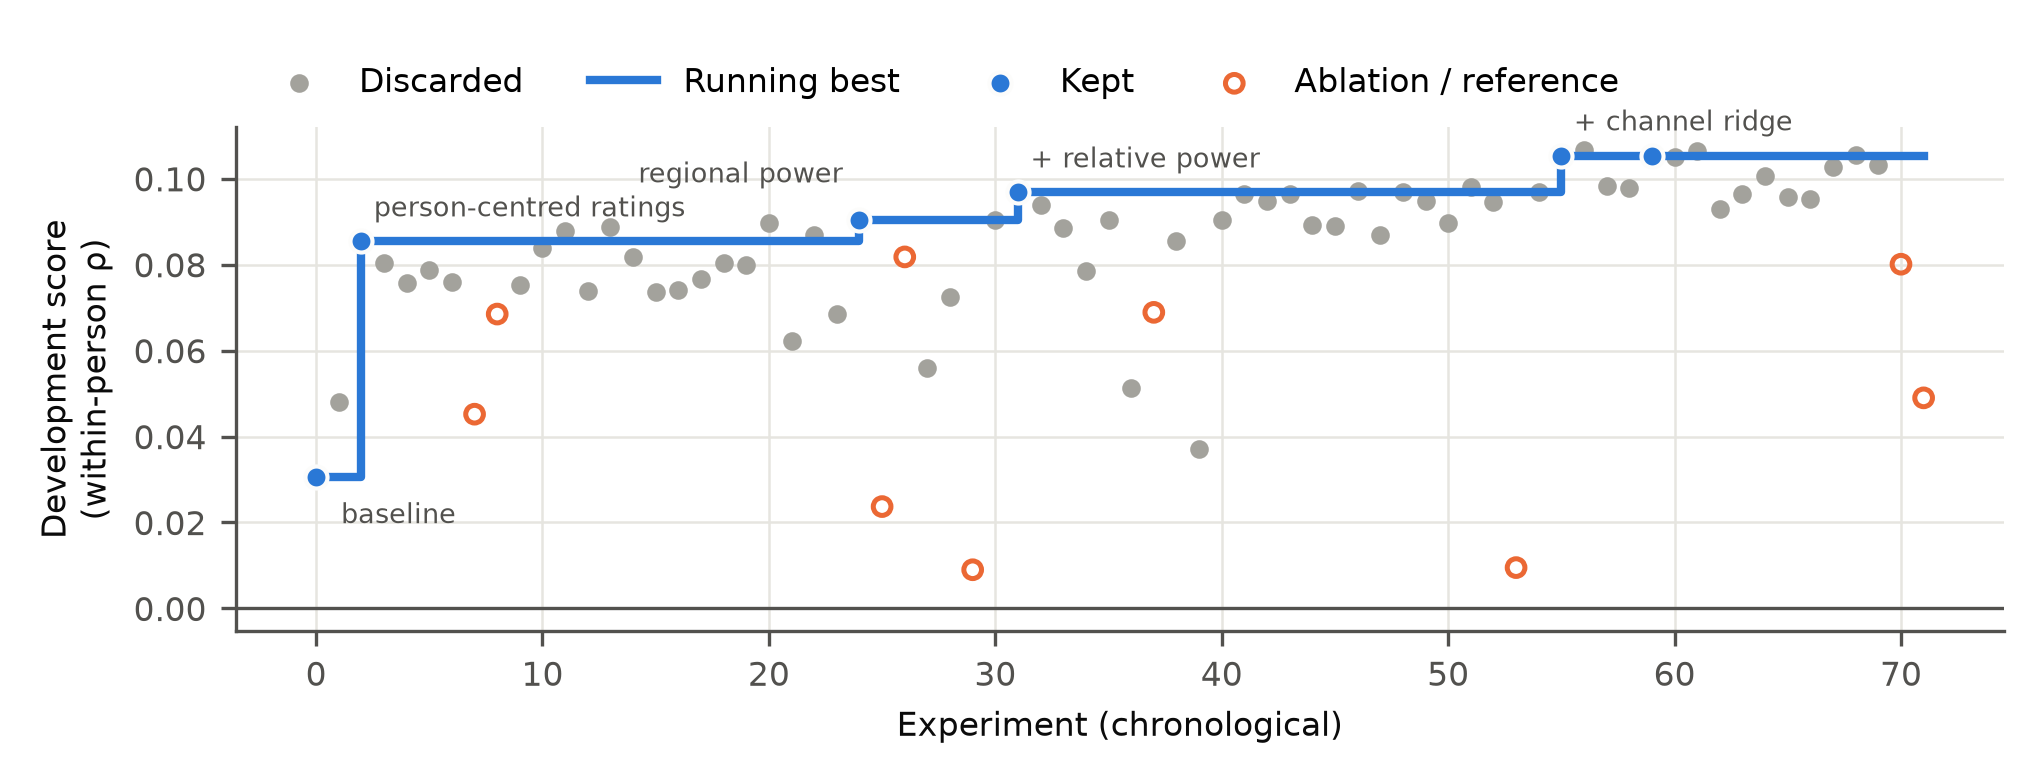
\includegraphics[width=\linewidth]{figures/progress.png}
\caption{Development score of the 72 experiments in order. Blue points are
kept changes; the line is the running best. Open orange circles are
ablations and references, never kept.}
\label{fig:progress}
\end{figure}

\paragraph{Sealed test.} Table~\ref{tab:test} and Figure~\ref{fig:test}
give the sealed results. In the primary regime the final model scored 0.139
(0.083 to 0.196), against 0.083 (0.031 to 0.136) for the starting model.
The paired gain of +0.056 (+0.012 to +0.101) excludes zero. Its development
counterpart was +0.075, so roughly a quarter of the gain did not carry over,
but the final model's own development score (0.105) sat below its test score.
With 55 test people and 21 test themes, the intervals are wide. The gain also
held for the two other regimes, at +0.035 (+0.009 to +0.061) for new people
with seen themes and +0.038 (+0.019 to +0.056) for seen people with new
themes.

\begin{table}[t]
\centering
\small
\begin{tabular}{lccc}
\toprule
 & New person, new theme & New person, seen theme & Seen person, new theme\\
 & 1,174 trials, 55 people & 2,760 trials, 55 people & 5,652 trials, 258 people\\
\midrule
Starting model & 0.083 [0.031, 0.136] & 0.117 [0.077, 0.159] & 0.069 [0.045, 0.092]\\
Final model & 0.139 [0.083, 0.196] & 0.152 [0.108, 0.196] & 0.106 [0.080, 0.133]\\
\quad EEG only & 0.100 [0.046, 0.153] & 0.118 [0.070, 0.166] & 0.077 [0.051, 0.103]\\
\quad Peripheral only & 0.126 [0.072, 0.185] & 0.076 [0.045, 0.109] & 0.082 [0.059, 0.105]\\
Session position only & 0.048 [$-$0.015, 0.108] & 0.027 [$-$0.019, 0.071] & 0.042 [0.017, 0.068]\\
\midrule
Final, pooled AUC (V/A) & 0.523 / 0.530 & 0.562 / 0.541 & 0.534 / 0.552\\
\bottomrule
\end{tabular}
\caption{Sealed-test score (within-person $\rho$, mean of valence and
arousal) with 95\% person-bootstrap intervals. All models were fitted once on
the 13,388 development trials.}
\label{tab:test}
\end{table}

\begin{figure}[t]
\centering
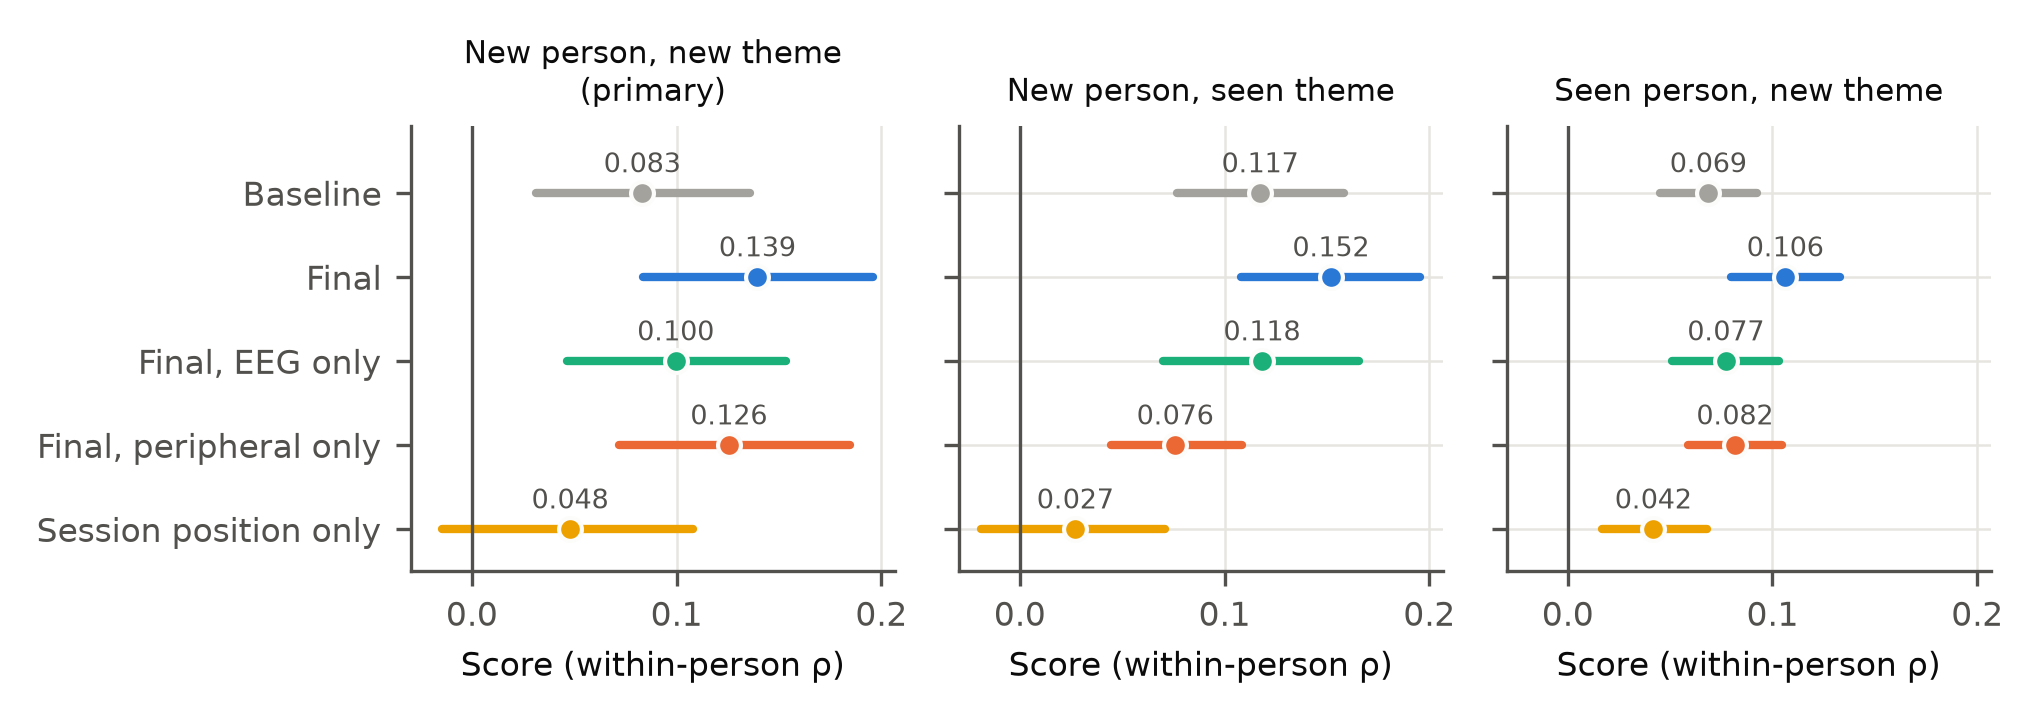
\includegraphics[width=\linewidth]{figures/sealed_test.png}
\caption{Sealed-test scores with 95\% person-bootstrap intervals.}
\label{fig:test}
\end{figure}

\paragraph{Seen versus new videos.} For the final model, new people with seen
themes scored 0.152 and new people with new themes 0.139; for the starting
model, 0.117 and 0.083. These sets share the same 55 people, so the
difference is descriptive. Seeing the themes in training helped little once
ratings were centred per person. A stronger test came from development. A
model fitted on video means of person-centred features and ratings, which keeps
only the physiology common to all viewers of a video, scored 0.010 (interval
$-$0.007 to 0.026). What transfers to new themes is the individual response
to a trial.

\paragraph{Signals.} In development, the EEG-only version of the final model
predicted valence as well as the full model ($\rho$ = 0.108 versus 0.110)
but arousal poorly (0.053 versus 0.101). The peripheral-only version predicted
arousal (0.081) but not valence (0.017) (Figure~\ref{fig:signals}). On the
sealed test, peripheral signals alone also reached 0.095 for valence, an
estimate from 55 people that we read as noise around the development figure.
Gamma power alone scored 0.024 in development and removing it cost 0.004, so
facial muscle activity, which concentrates above 30 Hz, does not explain the
decoding. Session position alone scored 0.009 in development and 0.048 in the
primary test regime, with an interval that includes zero.

\begin{figure}[t]
\centering
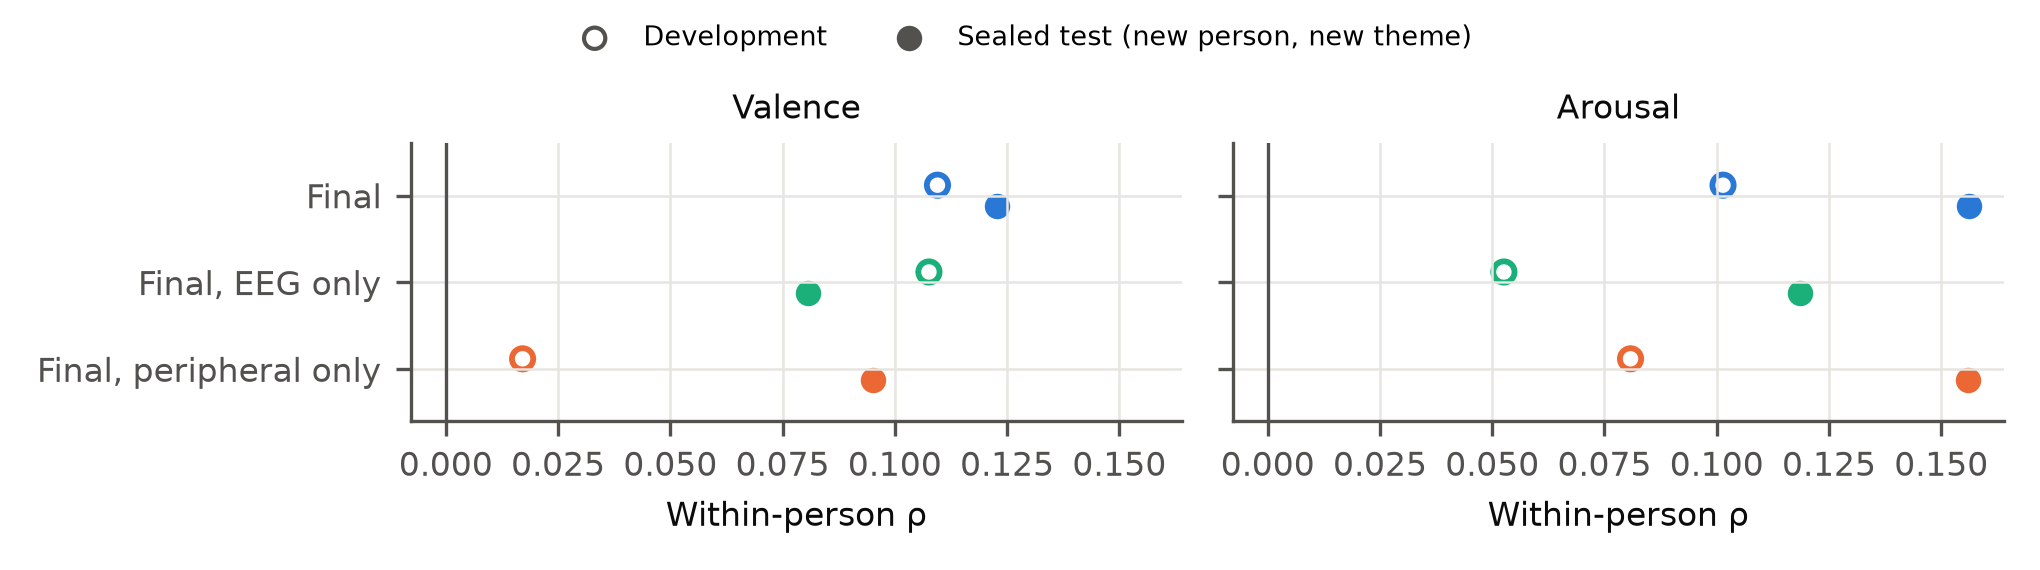
\includegraphics[width=\linewidth]{figures/modalities.png}
\caption{Within-person $\rho$ per rating for the final model and its two
ablations. Open circles: development cross-fit. Filled circles: sealed test,
new person and new theme.}
\label{fig:signals}
\end{figure}

\section{Discussion}

The search produced a model that a held-out test confirmed, with a gain whose
interval excludes zero. The changes that survived are simple. They centre the
target on the person, pool channels, add relative power and average two
linear models. More flexible models lost every comparison. The signal is weak and
mostly linear, and with about 6,000 training trials per fold, variance
dominates.

The effect is small. A within-person
correlation of 0.14 means the model orders a new viewer's trials slightly
better than chance. The pooled AUCs of 0.52 to 0.56 are lower than the 0.58
reported by another team, but the two numbers do not measure the same thing:
our predictions carry no person offset by construction, and that team's
split is unknown.

The sealed test addressed the main risk of autoresearch, selection on a
reused validation set. Seventy-two scored variants on the same development
blocks did not inflate the final development score above the test score,
although the gain shrank from 0.075 to 0.056. Two parts of the design may
explain why the optimism stayed small. The keep threshold rejected 57 changes, and the blocked
cross-fit scored every development trial with a model blind to its person
and theme.

\paragraph{Limitations.} The test set is one split of 55 people and 21
themes, and its intervals span about 0.11. The features are fixed. The agent
could not change extraction, so window length, filtering and time-resolved
features are untested. The final model scales each regression's output by
its spread over the predicted batch, which assumes a batch of trials from the
new person, without labels. Ratings are coarse 1 to 9 integers, and 76 trials
used non-ICA EEG. The agent wrote the variants in parallel batches, not one
at a time as in the original loop, and a human chose the objective, the
threshold and when to stop.

\paragraph{Reproducibility.} \texttt{autoresearch/} holds the extractor,
the fixed scorer, the final model and \texttt{program.md}.
\texttt{results.tsv} lists all 72 experiments with commit, score and
decision. The sealed metrics are in
\nolinkurl{docs/research/autoresearch/results/sealed_test.json} (GitHub Actions
run 44598712146). The repository publishes only aggregate numbers.

\paragraph{References.} A.~Karpathy, \emph{autoresearch},
github.com/karpathy/autoresearch, 2026. HABS team, dataset paper and
\texttt{DATASET.md}, HABS Neuro-AI Hackathon, 2026.

\end{document}
